\documentclass{beamer}

\mode<presentation>
{
  \usetheme{CambridgeUS}
  \setbeamercovered{transparent}
}

\usepackage[english]{babel}
\usepackage[latin1]{inputenc}
\usepackage{times}
\usepackage[T1]{fontenc} 
% Or whatever. Note that the encoding and the font should match. If T1
% does not look nice, try deleting the line with the fontenc.
\usepackage{amsmath}
\usepackage{algorithmic}

\newcommand{\linespace}{\vskip 0.25cm}

\definecolor{MyForestGreen}{rgb}{0,0.7,0} 
\newcommand{\tableemph}[1]{{#1}}
\newcommand{\tablewin}[1]{\tableemph{#1}}
\newcommand{\tablemid}[1]{\tableemph{#1}}
\newcommand{\tablelose}[1]{\tableemph{#1}}

\definecolor{MyLightGray}{rgb}{0.6,0.6,0.6}
\newcommand{\tabletie}[1]{\color{MyLightGray} {#1}}

% The text in square brackets is the short version of your title and will be used in the
% header/footer depending on your theme.
\title[Intrusion Detection]{Intrusion Detection with \\ Genetic Algorithms and Fuzzy Logic}

% Sub-titles are optional - uncomment and edit the next line if you want one.
% \subtitle{Why does sub-tree crossover work?} 

% The text in square brackets is the short version of your name(s) and will be used in the
% header/footer depending on your theme.
\author[Ireland]{Emma Ireland}

% The text in square brackets is the short version of your institution and will be used in the
% header/footer depending on your theme.
\institute[U of Minn, Morris]
{
  Division of Science and Mathematics \\
  University of Minnesota, Morris \\
  Morris, Minnesota, USA
}

% The text in square brackets is the short version of the date if you need that.
\date[December '13] % (optional)
{December 2013 \\ UMM CSci Senior Seminar Conference}

% Delete this, if you do not want the table of contents to pop up at
% the beginning of each subsection:
\AtBeginSection[]
{
  \begin{frame}<beamer>
    \frametitle{Outline}
    \tableofcontents[currentsection, hideothersubsections]
  \end{frame}
}

\begin{document}

\begin{frame}
  \titlepage
\end{frame}

% For a 20-25 minute senior seminar talk you probably want something like:
% - Two or three major sections (other than the summary).
% - At *most* three subsections per section.
% - Talk about 30s to 2min per frame. So there should probably be between
%   15 and 30 frames, all told.

\section*{Overview}

\subsection*{The Big Picture}

\begin{frame}
  \frametitle{The Big Picture}
  
  \begin{columns}
  \begin{column}{0.6\textwidth}
  \begin{itemize}
  	\item 
	\item 
	\item 
	\item 
	\item 
  \end{itemize}
  \end{column}
  \begin{column}{0.4\textwidth}
   
  \end{column}
  \end{columns}
\end{frame}

\subsection*{Outline}

\begin{frame}
  \frametitle{Outline}
  \tableofcontents[hideallsubsections]
\end{frame}
%%%%%%%%%%%%%%%%%%%%%%%%%%%%%%%%%%%%%%%%%%%%%%%%%%%%%%%%%%%%%%%%%%%%%%%%%%%%%%%%%
%%%%%%%%%%%%%%%%%%%%%%%%%%%%%%%%%%%%%%%%%%%%%%%%%%%%%%%%%%%%%%%%%%%%%%%%%%%%%%%%%
%%%%%%%%%%%%%%%%%%%%%%%%%%%%%%%%%%%%%%%%%%%%%%%%%%%%%%%%%%%%%%%%%%%%%%%%%%%%%%%%%
%%%%%%%%%%%%%%%%%%%%%%%%%%%%%%%%%%%%%%%%%%%%%%%%%%%%%%%%%%%%%%%%%%%%%%%%%%%%%%%%%
\section[Background]{Background}
\subsection{Types of Networking Attacks}
\begin{frame}
  \frametitle{Types of Networking Attacks}
Explain DoS, remote to user, user to root, probe
\end{frame}


\subsection{Detection Methodologies}
\begin{frame}
  \frametitle{Detection Methodologies}
Explain signature-based and anomaly-based detection
\end{frame}


\subsection{Data Sets - KDD99 and RLD09}
\begin{frame}
  \frametitle{KDD99}
	\begin{itemize}
		\item Generated by simulating a military network environment in 1999.
		\item Has long been a standard data set for intrusion detection.
		\item Data in the set is classified as normal or attack activity.
		\item KDD99 uses 41 features.
		\begin{itemize}
		  	\item \emph{Features} are properties of a \emph{record}, (either an attack or normal activity), that are used to describe the activity.
		\end{itemize}

	\end{itemize}
\end{frame}


\begin{frame}
  \frametitle{Some Features of KDD99}
	\begin{itemize}
		\item duration: length of the normal or attack activity
in seconds.
		%\item src\_bytes: number of bytes sent from source to destination.
		\item num\_failed\_logins: number of failed login attempts.
		\item root\_shell: returns 1 if root shell is obtained, else returns 0.
		%\item num\_access\_files: number of operations on access control files.
		%\item srv\_count: number of connections to the same service as the current connection in the past two seconds.
		\item serror\_rate: percentage of connections that have ``SYN" errors.
		%\item same\_srv\_rate: percentage of connections to the same service.
	\end{itemize}
\end{frame}



\begin{frame}
  \frametitle{RLD09}
	\begin{itemize}
		\item RLD09 was created because KDD99 is 14 years old.
		\item Data was captured from a university in Bangkok, Thailand.
		\item The data has 10 million data packets, 17 different types of attacks (divided into denial of service and probe attacks), and 12 features.
	\end{itemize}
\end{frame}


\subsection{Rules}
\begin{frame}
  \frametitle{Rules}
	\begin{itemize}
		\item Elements of one set are separated into different sets in order to differentiate between normal connections and attacks.
		\item If-Then format
		\begin{itemize}
			\item If the length of the activity is 4 seconds, then the probability of it being an attack is 100\%.
		\end{itemize}				
	\end{itemize}
\end{frame}


\subsection{Genetic Algorithms}
\begin{frame}
  \frametitle{Genetic Algorithms}

\end{frame}


\subsection{Determining the Accuracy of an Algorithm}
\begin{frame}
  \frametitle{Determining the Accuracy of an Algorithm}
	\begin{itemize}
		\item False positive (FP): intrusion detection system incorrectly identifies normal activity as being an attack. 
		\item False negative (FN): intrusion detection system fails to identify harmful activity. 
		\item True positive (TP): intrusion detection system correctly identifies activities to be attacks. 
		\item True negative (TN): intrusion detection system correctly
identifies activities to be normal.
		\item Detection rate (DR): the number of true positives divided by the total number of intrusions that happen.
	\end{itemize}
\end{frame}
%%%%%%%%%%%%%%%%%%%%%%%%%%%%%%%%%%%%%%%%%%%%%%%%%%%%%%%%%%%%%%%%%%%%%%%%%%%%%%%%%
%%%%%%%%%%%%%%%%%%%%%%%%%%%%%%%%%%%%%%%%%%%%%%%%%%%%%%%%%%%%%%%%%%%%%%%%%%%%%%%%%
%%%%%%%%%%%%%%%%%%%%%%%%%%%%%%%%%%%%%%%%%%%%%%%%%%%%%%%%%%%%%%%%%%%%%%%%%%%%%%%%%
%%%%%%%%%%%%%%%%%%%%%%%%%%%%%%%%%%%%%%%%%%%%%%%%%%%%%%%%%%%%%%%%%%%%%%%%%%%%%%%%%
\section[Genetic Algorithm Implementation]{Genetic Algorithm Implementation}
\subsection{Algorithm Overview}
\begin{frame}
  \frametitle{Algorithm Overview}

\end{frame}


\subsection{Experimental Design and Results}
\begin{frame}
  \frametitle{Experimental Design}

\end{frame}


\begin{frame}
  \frametitle{Results}

\end{frame}
%%%%%%%%%%%%%%%%%%%%%%%%%%%%%%%%%%%%%%%%%%%%%%%%%%%%%%%%%%%%%%%%%%%%%%%%%%%%%%%%%
%%%%%%%%%%%%%%%%%%%%%%%%%%%%%%%%%%%%%%%%%%%%%%%%%%%%%%%%%%%%%%%%%%%%%%%%%%%%%%%%%
%%%%%%%%%%%%%%%%%%%%%%%%%%%%%%%%%%%%%%%%%%%%%%%%%%%%%%%%%%%%%%%%%%%%%%%%%%%%%%%%%
%%%%%%%%%%%%%%%%%%%%%%%%%%%%%%%%%%%%%%%%%%%%%%%%%%%%%%%%%%%%%%%%%%%%%%%%%%%%%%%%%
\section[Fuzzy Genetic Algorithm Implementation]{Fuzzy Genetic Algorithm Implementation}

\subsection{Fuzzy Algorithm}

\begin{frame}
  \frametitle{Measuring the Probability of a Record Being an Attack}

  \begin{columns}
  \begin{column}{0.6\textwidth}
  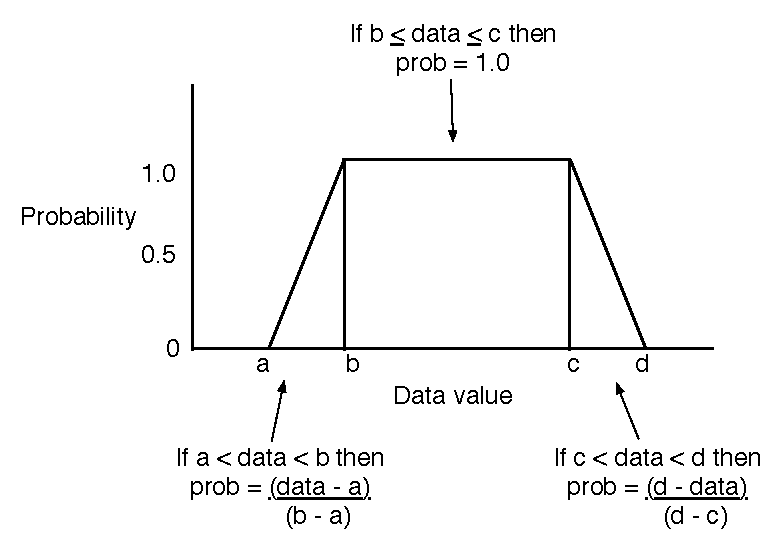
\includegraphics[width=0.95\textwidth]{../TrapezoidFigure.pdf}
  \end{column}

  \begin{column}{0.4\textwidth}
  Example:
  \begin{itemize}
  	\item Feature: duration (length of the activity in seconds).
  	\item a=1, b=3, c=5, d=7
  	\item The length of the activity is 6 seconds (between c and d).
  	\linespace
  	\item prob = $\frac{d-\textrm{data}}{d-c}$ = $\frac{7-6}{7-5}$ = 0.5
  \end{itemize}

  \end{column}
  \end{columns}
\end{frame}


\begin{frame}
	\frametitle{Encoding of Features and Rules}
	\begin{itemize}
	\item The four parameters are encoded into blocks.
	\item Each block is a feature with values between 0.0 and 7.0.
	\end{itemize}
	
\begin{figure}
\begin{tabular}{|cccc|} \hline
010 & 011 & 100 & 101\\
a=2 & b=3 & c=4 & d=5\\
\hline\end{tabular}
\end{figure}

	\begin{itemize}
	\item A rule has 12 blocks of features, at the end is the type of attack.
	\end{itemize}

\begin{figure}
\begin{tabular}{|cccc|c|cccc|c|} \hline
010 & 011 & 100 & 101   & ...... & 010 & 011 & 101 & 111   & DoS\\
a=2 & b=3 & c=4 & d=5   & ...... & a=2 & b=3 & c=5 & d=7   &\\ 
    &     & Block 1&    &        &     & Block 12& &       & Type\\
\hline\end{tabular}
\end{figure}

\end{frame}


\subsection{Algorithm Overview}

\begin{frame}
	\frametitle{Algorithm Overview}
\begin{columns}
\begin{column}{0.6\textwidth}
\begin{algorithmic}
\FOR{each record}
  \FOR{each rule}
    \FOR{each feature}
      \STATE{prob = fuzzy(); // Trapezoidal fuzzy rule shape}
      \STATE{totalprob = totalprob + prob;}
    \ENDFOR    
    \IF{totalprob > threshold} 
      \STATE{class is attack;}
      %\ELSE \STATE{class is normal;}
    \ENDIF
  \ENDFOR
  \STATE{find $A$, $B$, $\alpha$, and $\beta$  %// $A$: \# of attack records. $B$: \# of normal records. $\alpha$: \# of attack records correctly identified as attack. $\beta$: \# of normal records incorrectly classified as attack.}
  
  } 
\ENDFOR
\STATE{calculate fitness}
\STATE{crossover(), mutation()}

\end{algorithmic}
\end{column}

\begin{column}{0.4\textwidth}
	Fitness function:
	\begin{equation*}
	\frac{\alpha}{A} - \frac{\beta}{B}
	\end{equation*}

	$A$: \# of attack records.
	
	$B$: \# of normal records. 

	$\alpha$: \# of attack records correctly identified as attack.

	$\beta$: \# of normal records incorrectly classified as attack.
	
\end{column}
\end{columns}
\end{frame}


\subsection{Experimental Design and Results}

\begin{frame}
	\frametitle{Experiments}
	\begin{itemize}
		\item A variety of experiments were run. Two experiments used just RLD09, and three experiments used KDD99 and RLD09 together.
		\item The experiments used a total of 16,000 records of normal activity and 10,500 records of attack activity. Of the attack records, 4,000 were denial of service attacks and 6,500 were probe attacks.
	\end{itemize}
\end{frame}


\begin{frame}
	\frametitle{Experiments Using Only RLD09}
Experiment 1
\end{frame}


\begin{frame}
	\frametitle{Experiments Using Only RLD09}
Experiment 2
	
\end{frame}


\begin{frame}
	\frametitle{Experiments Using Both RLD09 and KDD99}
Experiment 1
	
\end{frame}


\begin{frame}
	\frametitle{Experiments Using Both RLD09 and KDD99}
Experiment 2
	
\end{frame}


\begin{frame}
	\frametitle{Experiments Using Both RLD09 and KDD99}
Experiment 3
	
\end{frame}
%%%%%%%%%%%%%%%%%%%%%%%%%%%%%%%%%%%%%%%%%%%%%%%%%%%%%%%%%%%%%%%%%%%%%%%%%%%%%%%%%
%%%%%%%%%%%%%%%%%%%%%%%%%%%%%%%%%%%%%%%%%%%%%%%%%%%%%%%%%%%%%%%%%%%%%%%%%%%%%%%%%
%%%%%%%%%%%%%%%%%%%%%%%%%%%%%%%%%%%%%%%%%%%%%%%%%%%%%%%%%%%%%%%%%%%%%%%%%%%%%%%%%
%%%%%%%%%%%%%%%%%%%%%%%%%%%%%%%%%%%%%%%%%%%%%%%%%%%%%%%%%%%%%%%%%%%%%%%%%%%%%%%%%
\section[Conclusions]{Conclusions}

\begin{frame}
\frametitle{Conclusions}

\begin{itemize}
  \item 
  
  \linespace
  
  \item 

  \linespace
  
  \item
\end{itemize}


\end{frame}

\begin{frame}
	\frametitle{Thanks!}
	
	Thank you for your time and attention!
		
	\linespace
	\linespace
	
	\begin{center}
	{\huge Questions?}
	\end{center}
\end{frame}

\section*{References}

\begin{frame} 
	\frametitle{References} 
	
	\begin{thebibliography}{lskdjf}
	
  	\end{thebibliography}
	
\end{frame} 

\end{document}


